%!TEX root = main.tex
\begin{figure}
	\centering
	\scalebox{.5}{
	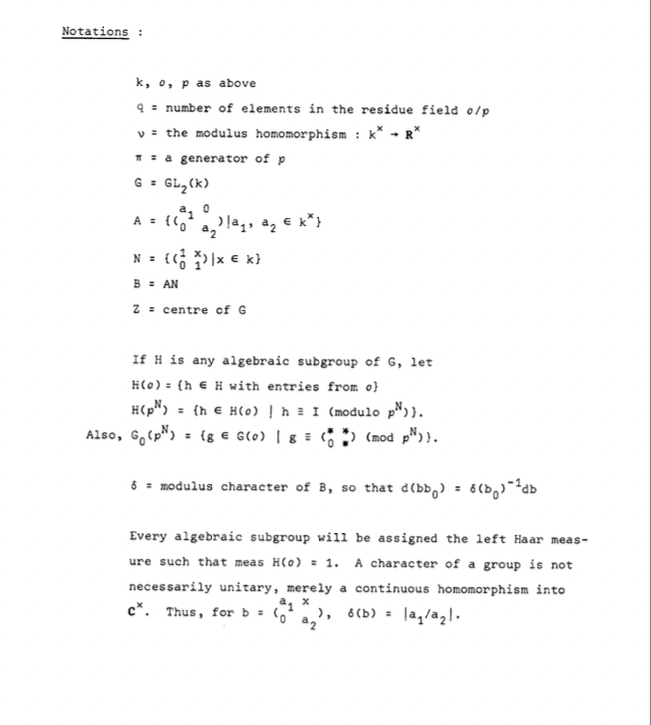
\includegraphics{
	branch-decompositions-notation.png}
	}
\end{figure}

An admissible rep of $G$ is complex vector space $V$ and a $\rho : G \to \Aut(V)$ such that 
\begin{itemize}
	\item For all $v\in V$, the stabilizer of $v$ in $G$ is an open subgroup; this is needed for matrix coefficients of $V$ to be \emph{locally constant}. This is smoothness
	\item For each compact open subgroup $K\leq G,$ the $K$-fixed vectors $V^K$ form a finite dimensional subspace.
\end{itemize}

For a character $\mu :A \to \C^\times$, extend $\mu$ to $B=NA$ so that $\mu(n) =1$ for all $n\in N$, and define the space of $\Ind(\mu)$ to be the space of locally constant functions $f: G \to \C$ such that $f(n a g) = \delta^{1/2}(n a)\mu(n a)f(g)$. 



% For a group $G$ and a subgroup $H\leq G$, let $\pi : G \epi G/H$ be the canonical projection. Then $G$ is a principal $H$ bundle over $G/H$; this is tautological.

% Let $s: G/H \to G$ be a section (supposing one exists in the relevent category).  

% Given a representation $\rho$ of $H$ on a space $V$. The associated bundle is $G\times V \rmod (g,v) \sim (gh, \rho(h^\inv ) v) := G \times_H V \epi G/H$    via $\pi(g,v) = g H$. I.e.: sitting above each point $gH \in G/H$ is a copy of $V$.  

\def\Map{\rm Map}
% Let 
% \[
% \Map_H(G,V) = \{ f: G \to V \vert f(gh) = \rho(h^\inv) f(g)\, , (g,h) \in G\times H \}.
% \]

% This space of $V$ valued functions on $G$ can be identified with the space $\Gamma(E_V)=\Gamma(G,H,V)$ of sections $s: G/H \to E_V = G\times_H V$. Explicitly, given $f\in \Map_H(G,V)$, define a section $s$ by $s(gH)=(g,f(g)).$

In the description of $\Ind_B^G(\mu)$ as a space of functions on $G$ which are $(B,\mu)$  equivariant, view all of the $\Ind_B^G(\mu)$ as living inside some suitably large space of complex valued functions on $G$. One can do this in such a way that there is a consistent action of $G$ on functions \emph{by translation}. Other models substitute, for example, a consistent action for a consistent underlying space of functions. 

Keeping notation consistent with Bill's, $PS(\mu)$ is the principal series, and is associated to a $\mu : A \to \C^\times$. 

The definition of admissibility is designed so that the contragredient representation $\tilde{\rho}$ of admissible $\rho$ is admissible. The underlying space of $\tilde{\rho}$ is the collection of linear functionals on $\rho$ which are fixed by some open subgroup of $G$.

Integration yields a hermitian pairing $PS(\mu)\times PS(\mu^\inv ) \to \C$, so that $PS(\mu^\inv)$ is the contragredient to $PS(\mu)$. The underlying mechanism is that there is a unique $G$ invariant linear functional $I$ on $\Ind(\delta^{1/2})$ such that on the subspace of smooth compactly supported function $f: G \to \C$, one has $I(P_\delta f(g)) = \int_G f(g) \dop g$, where $P_\delta f(g) = \int _B f(bg) \dop b. $

Given an admissible representation $\rho$ of $G$ on a space $V$, set 
\[
	V(N) = \{ v  :  \int_\bfrak \rho(\tbt{1}{x}{0}{1} ) v \dop x = 0  \text{ some fractional ideal } \bfrak \}.
\]


% \subsection{Some comments on choices}
% Briefly lets let $\kfrak$ be algebraically closed, and $G=\GL(V)$ where $V$ is a two dimensional vectorspace over $\kfrak$

% Picking a maximal torus $T$ in $G$ amounts to picking a pair of linearly independent lines in $V.$ Note, this is not quite the same as picking a basis. These lines are the common eigenspaces of every element of $T$. 

% Picking (one of the two possible) orderings on the two roots of $T$ in $G$ amounts to a choice of borel $B$ containing $T$.  
\def\Aff{\rm Aff}
\section{Cartan Decomposition}
Let $G$ act on the set of ordered bases of $\kfrak^2$ by letting $g=\tbt{a}{b}{c}{d}$ send $(e_1,e_2)$ to $(ae_1 +b e_2 , ce_1 +de_2).$ 

Given an ordered basis $(e_1,e_2)$, let $\langle e_1,e_2\rangle = \ofrak e_1 + \ofrak e_2  \leq \kfrak^2$ be the lattice generated by it. 

Let $L=\langle u_1,u_2 \rangle $ be the lattice generated by the standard basis and $L'= gL$ the lattice generated by $g(u_1,u_2).$

Elementary divisor theorem implies there exists an $\ofrak$ basis $(v_1,v_2)$ of $L$ and elements $a_1,a_2 \in \kfrak^\times $ with $a_1 \in \ofrak a_2$ such that $(a_1v_1,a_2v_2)$ is a basis for $L'$. 

That is, there exists a $k_1 \in \GL_2(\ofrak)$ sending $(u_1,u_2)$ to $(v_1,v_2)$, and another $k_2 \in \GL_2(\ofrak)$ such that $k_2 g(u_1,u_2) = (a_1 v_1, a_2 v_2).$ If $a = \tbt{a_1}{}{}{a_2}$ then $k_2 g = a k_1$.  

Leting $A^{-}  = \{\tbt{a_1}{}{}{a_2}: \, a_1 \in a_2 \ofrak \}$, we have shown
\[ \boxed{
\GL_2(\kfrak) = \GL_2(\ofrak) \cdot A^{-} \cdot \GL_2(\ofrak), 
}\]

\section{Iwasawa decomposition} 
$\GL_2(\kfrak)$ acts transitively on $\Pbb^1(\kfrak)$. The stabilizer of any point is conjugate to the standard borel $B(\kfrak)$ of upper triangulars (equivalently, any point in $\Pbb^1$ can be taken to $\infty$).

Restricting the surjection $G(\kfrak) \to G(\kfrak) / B(\kfrak) = \Pbb^1(\kfrak)$ to $G(\ofrak)$ remains surjective, and induces an identification of $G(\ofrak) / B(\ofrak)$ with $\Pbb^1(\kfrak)$. 

\section{Iwahori factorization}
Every element $g \in G_o(\pfrak)$ has a unique decomposition $n^{-} b$ with $n^{-} \in N^{-}(\pfrak)$ and $b\in B(\ofrak)$:
\[ 
	\boxed{
		G_o(\pfrak) = N^{-} (\pfrak) B(\ofrak). 
	}
\]

Indeed, if $c\in \pfrak$ then $a \in \ofrak^\times$  and 
\[ \Tbt{a}{b}{c}{d} = \Tbt{1}{0}{c/a}{1} \cdot   \Tbt{a}{b}{0}{d-bc/a} \]